\section{Principal-seven transport and its complete divisor}\label{sec:principal}
\noindent\textit{Source anchor P: v0.12--v0.13 principal-seven and divisor proofs. The formulas are typeset in mathematical notation; the source originals remain intact.}

\subsection{The seven-point product}
Use the fixed periods of Section~\ref{sec:setting}. Define
\[
 S_5(z;a,b)=\frac{\Gamma_{\rm ell}(z;a,b)^5}
 {\Gamma_{\rm ell}(5z;5a,5b)},\qquad
 F(z)=S_5(z+t;t,s)^{-1}.
\]
All identities below are meromorphic identities; their quotients at apparent exceptional points mean meromorphic continuation. Let
\[
 \Lambda_5=\mathbb Z\tau+\mathbb Zs+\tfrac15\mathbb Z,
 \qquad \delta=\frac{\tau+2s+4}{7}.
\]
The period identities, obtained from $\beta^3=7$, are
\begin{equation}\label{eq:period-identities}
\begin{aligned}
 \beta\tau&=2\tau+4s+1,&\beta s&=-\tau,&\beta&=-15s-2,\\
 \beta\delta&=-8s-1,&7\delta&=\tau+2s+4.
\end{aligned}
\end{equation}
The seven-point product and its correction are
\begin{equation}\label{eq:p7}
 P_7(z)=\prod_{k=0}^{6}F(z+k\delta)
 =\frac{S_5(z;s,\delta)}{S_5(z;t,\delta)S_5(z+s;t,\delta)},
 \qquad R(z)=\frac{P_7(z)}{F(\beta z)}.
\end{equation}
The product identity is an actual gamma multiplication identity, not the assertion $P_7(z)=F(\beta z)$. For completeness, its elementary product proof is retained from v0.12: rewrite $t=2s+4-7\delta$, regard periods modulo integers, and perform real root averaging and vertical residue splitting in the defining gamma products. The resulting split factors are precisely $S_5(z;s,\delta)$, $S_5(z;t,\delta)^{-1}$ and $S_5(z+s;t,\delta)^{-1}$. The full source derivation and its positive-period convention are reproduced in Appendix~\ref{sec:seven-product-proof}. No scalar inferred from a numerical sample is inserted.

\par
\begin{figure}[htbp]\centering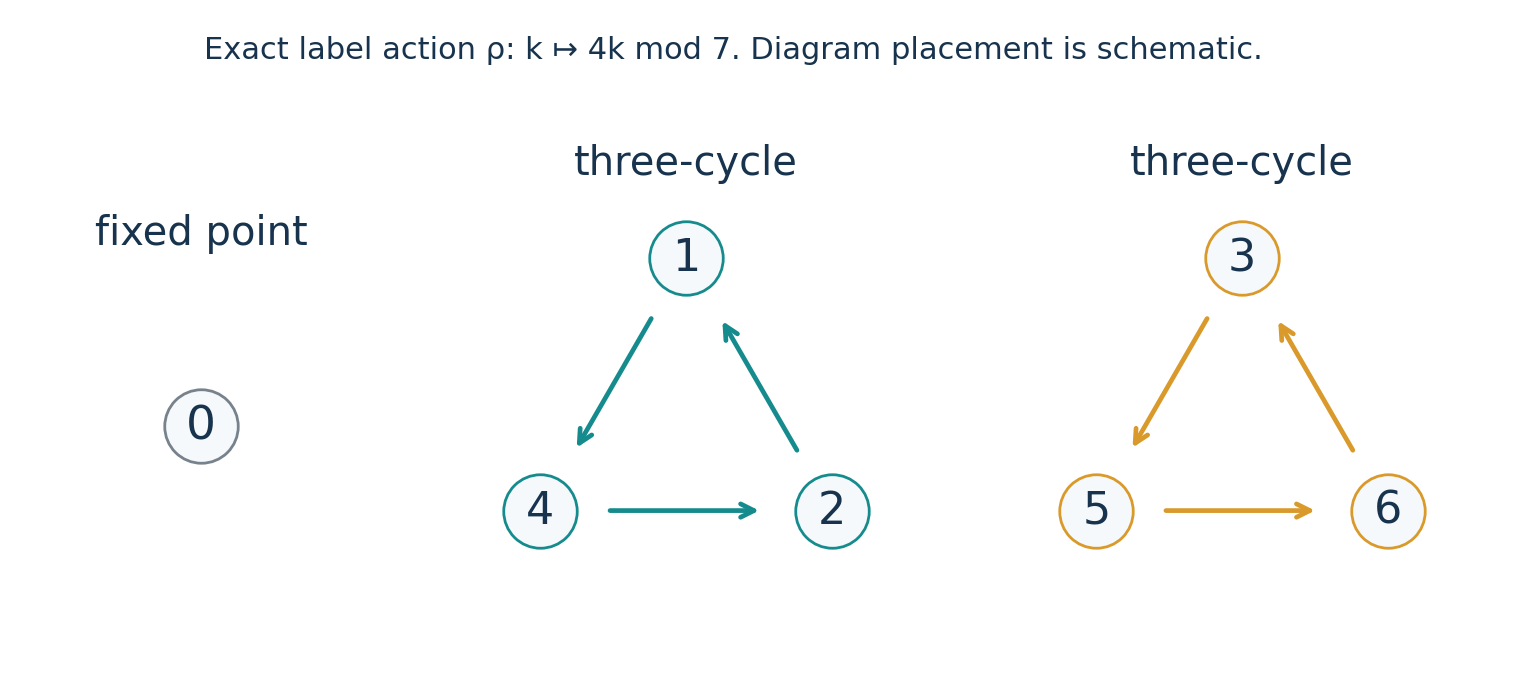
\includegraphics[width=.92\linewidth]{figures/04_seven_cover.png}\caption{The exact action of the inverse unit on the seven cover labels is $k\mapsto4k\pmod7$. The diagram places the fixed label and two three-cycles schematically; representative transport retains its theta carries.}\label{fig:cover}\end{figure}
\par

\subsection{Base divisor and the integral lift}
Define
\[
 H(n)=\mathbf1_{\{n>0\}},\qquad
 w(c)=\begin{cases}4,&5\mid c,\\-1,&5\nmid c.\end{cases}
\]
The function $H$ here is an integer step function, distinct from the eta quotient $\mathcal H$ and the locally defined CM Green quantity $H(z)$ used elsewhere.

\begin{theorem}[Base half-space divisor]\label{thm:base-divisor}
The divisor of $F$ is supported on $\Lambda_5$. At its uniquely parametrized point,
\begin{equation}\label{eq:base-divisor}
 \operatorname{ord}_{a\tau+bs+c/5}F=w(c)\,[H(a)-H(b)].
\end{equation}
\end{theorem}
\begin{proof}
For positive periods $t,s$, the defining gamma product has a simple zero at $jt+ks+\mathbb Z$ for $j,k\ge1$, a simple pole for $j,k\le0$, and no divisor in the mixed cones. Rational independence of $1,t,s$ prevents collisions. The argument $z+t$ has coordinates $(1-a,b)$ in the $(t,s)$ basis, giving gamma order $H(b)-H(a)$. In
\[
 F(z)=\frac{\Gamma_{\rm ell}(5(z+t);5t,5s)}
 {\Gamma_{\rm ell}(z+t;t,s)^5},
\]
the numerator contributes for every integer $c$ and the denominator only when $5\mid c$. Their difference is \eqref{eq:base-divisor}. The same product lists all possible zeros and poles.
\end{proof}
The rank-three additive group $\Lambda_5\subset\mathbb C$ is nondiscrete. This does not make the divisor dense: its selected nonzero coefficients have locally finite support.

Multiplication by $\beta$ in the ordered basis $(\tau,s,1/5)$ is
\[
 N_5=\begin{pmatrix}2&-1&0\\4&0&-3\\5&0&-2\end{pmatrix},\qquad
 N_5^3=7I,\quad\det N_5=7,\quad
 N_5^{-1}=\frac17\begin{pmatrix}0&-2&3\\-7&-4&6\\0&-5&4\end{pmatrix}.
\]
Its quotient generator is $(1,2,20)/7$, representing $\delta$. Thus
\[
 \beta^{-1}\Lambda_5=\Lambda_5+\mathbb Z\delta.
\]
Write a potential singular point as
\begin{equation}\label{eq:lambda}
 \lambda(a,b,c)=\frac{a\tau+bs+c/5}{\beta},\qquad
 p=\left\lceil\frac{3c-2b}{7}\right\rceil,\qquad
 k=7p+2b-3c\in\{0,\ldots,6\}.
\end{equation}
Exactly one argument $\lambda+k\delta$ lies in $\Lambda_5$. Its integral coordinates are
\begin{equation}\label{eq:lift}
 (\widehat a,\widehat b,\widehat c)=(p,2p-a,20p+5b-8c).
\end{equation}
Indeed $N_5(\widehat a,\widehat b,\widehat c)^T=(a,b-8k,c-5k)^T$, which expresses $\beta(\lambda+k\delta)=\beta\lambda+k(-8s-1)$. The other six digits fail integrality. Also
\[
 \widehat c-2c=5(4p+b-2c),\qquad w(\widehat c)=w(c).
\]
This transports the fifth-smoothing weight exactly.

\begin{theorem}[Complete ceiling divisor]\label{thm:complete-divisor}
There are no zeros or poles of $R$ outside $\beta^{-1}\Lambda_5$. At \eqref{eq:lambda},
\begin{equation}\label{eq:complete-divisor}
 m_\lambda:=\operatorname{ord}_{\lambda}R
 =w(c)\,[H(p)-H(2p-a)-H(a)+H(b)]\in\{-4,-1,0,1,4\}.
\end{equation}
\end{theorem}
\begin{proof}
Apply Theorem~\ref{thm:base-divisor} at the unique integral numerator lift \eqref{eq:lift} and subtract the denominator order at $\beta\lambda$. The weights agree. To bound the bracket, when $a\le0,p>0$ it is $H(b)$; when $a>0,p\le0$ it is $H(b)-1$. In the other cases it is a difference of two zero-one values. Thus it lies in $\{-1,0,1\}$.
\end{proof}
In particular,
\[
 \operatorname{ord}_{n\tau}R=4\quad(n\ge1),\qquad
 \operatorname{ord}_{ns}R=-4\quad(n\in\mathbb Z\setminus\{0\}),\qquad
 \operatorname{ord}_{-n}R=4\quad(n\ge1).
\]
For these assertions the triples are $(2n,4n,5n)$, $(-n,0,0)$ and $(0,15n,10n)$ respectively. At zero the order is zero. Lean verifies the integer identities; the interpretation as complex orders is the ordinary product argument.

\subsection{All transition multipliers and the scalar anchor}
\begin{theorem}[Theta transitions]\label{thm:transitions}
The following hold meromorphically:
\begin{align}
 K(z):=\frac{R(z+1)}{R(z)}&=\prod_{r=1}^{15}q_t(\beta z-rs)^{-1},\label{eq:K}\\
 \frac{R(z+s)}{R(z)}&=\frac{q_s(\beta z-\tau)}{\prod_{k=0}^{6}q_t(z+k\delta)},\label{eq:Rs}\\
 \frac{R(z+\tau)}{R(z)}&=
 \frac{\prod_{k=0}^{6}q_s(z+k\delta)\prod_{r=0}^{3}q_t(\beta z+rs)}
 {q_s(\beta z)q_s(\beta z+\tau)},\label{eq:Rtau}\\
 \frac{R(z+\delta)}{R(z)}&=
 \frac{q_s(z)}{q_t(z)q_t(z+s)\prod_{r=1}^{8}q_t(\beta z-rs)}.\label{eq:Rdelta}
\end{align}
\end{theorem}
\begin{proof}
Use $F(z+1)=F(z)$, $F(z+\tau)/F(z)=q_s(z)$ and $F(z+s)/F(z)=q_t(z)^{-1}$. For \eqref{eq:K}, $P_7$ is period one and $\beta=-15s-2$, producing fifteen negative $s$ shifts in the denominator. For \eqref{eq:Rs} use $\beta s=-\tau$. For \eqref{eq:Rtau}, $\beta\tau=2\tau+4s+1$ gives two $q_s$ factors and four reciprocal $q_t$ factors; the $2\tau$ shift disappears from $q_t$ by ellipticity. Finally $P_7(z+\delta)/P_7(z)=F(z+7\delta)/F(z)$ and the last two identities of \eqref{eq:period-identities} give \eqref{eq:Rdelta}.
\end{proof}
Under $z\mapsto z+1$ the triple changes to $(a,b-15,c-10)$, leaving $p$ and $w(c)$ unchanged. Formula~\eqref{eq:complete-divisor} gives
\[
 \operatorname{ord}_{z+1}R-\operatorname{ord}_zR
 =-w(c)\mathbf1_{\{1\le b\le15\}},
\]
the divisor of \eqref{eq:K}. Under $z\mapsto z+\delta$ the triple becomes $(a,b-8,c-5)$; its digit decreases by one modulo seven, and its pivot increases exactly when the old digit is zero. These universal carry statements include negative coordinates.

\begin{theorem}[Three-theta anchor]\label{thm:anchor}
$R$ is regular and nonzero at zero, and
\begin{equation}\label{eq:R0}
 R_0:=R(0)=\prod_{j=0}^{2}q_t(u_j)^{-1},\qquad
 u_j=\frac{t+\delta}{2}+j\delta.
\end{equation}
\end{theorem}
\begin{proof}
Let $\mathcal H(a)=\eta(5a)/\eta(a)^5$. Direct product cancellation gives
\[
 S_5(z;a,b)\sim\frac5{(2\pi)^4}\mathcal H(a)\mathcal H(b)z^{-4}.
\]
The ratio in \eqref{eq:p7} therefore has value $P_7(0)=[\mathcal H(s)/\mathcal H(t)]/S_5(s;t,\delta)$. Since $F(0)=\mathcal H(s)/\mathcal H(t)=\epsilon^2$, the eta factors cancel and $R_0=S_5(s;t,\delta)^{-1}$. The period relation is $s=(t+\delta)/2+3\delta-2$. At the central point, $S_5((t+\delta)/2;t,\delta)=1$ by termwise coincidence of the gamma numerator and denominator factors, at both scales. Three positive $\delta$ shifts now give \eqref{eq:R0}. The three arguments have $s$ coefficients $1/7,3/7,5/7$ relative to $(1,t,s)$ and thus avoid the divisor of $q_t$.
\end{proof}
A nonzero meromorphic function with transitions \eqref{eq:K}, \eqref{eq:Rs}, \eqref{eq:Rdelta} and anchor \eqref{eq:R0} equals $R$. Its ratio with $R$ has periods $1,s,\delta$. Their rational independence makes this rank-three subgroup nondiscrete. Arbitrarily small nonzero periods force the derivative to vanish at every regular point; hence the ratio is constant, and its value at zero is one. This is analytic uniqueness, not an arithmetic evaluation at $1/3$.

\subsection{The conjugation divisor cannot be discarded}
Put $R^\#(z)=\overline{R(\overline z)}$. The cubic fields $\mathbb Q(\beta)$ and $\mathbb Q(\overline\beta)$ are distinct: equality would put $\beta/\overline\beta=\omega$ in a cubic field. Their intersection is $\mathbb Q$. The support of $\operatorname{div}R$ lies in the first, and that of $R^\#$ in the second. Since $\tau$ is irrational (indeed $\beta=2-1/(4+15\tau)$),
\[
 \operatorname{ord}_{\tau}(R/R^\#)=4.
\]
Thus this naive conjugation quotient is not a holomorphic unit. A constant polarization, root of unity or nowhere-zero holomorphic gauge cannot change this order. A relative scalar model must match the complete divisor, beginning with order four at $\tau$; agreement at this one point alone is insufficient. Divisor matching on $\mathbb C$ also does not supply torus periodicity or a principal-norm coboundary. The special-value reality problem at the rational point $1/3$ remains separate.
